\documentclass[review]{igs}

\usepackage[T1]{fontenc}
\usepackage[utf8]{inputenc}
\usepackage{microtype}
\usepackage[english]{babel}
\usepackage{amsmath,amssymb,mathtools,bm}
\usepackage{booktabs,tabularx,array}
\usepackage{graphicx}
\usepackage{enumitem}
\usepackage[authoryear,round]{igsnatbib}

\title[Isochrone overturning]{Isochrone overturning in steady glacier flow}
\author[Lipovsky]{Bradley Paul LIPOVSKY}
\affiliation{Department of Earth and Space Sciences, University of Washington, Seattle, USA\\
Correspondence: Bradley Paul Lipovsky, \texttt{bpl7@uw.edu}}

\begin{document}
\abstract{Ancient ice recovered at Allan Hills extends into the Miocene, but steep layers, age reversals and folds complicate its interpretation. Whether steady glacier flow can overturn initially ordered layers remains uncertain. Here, we track the horizontal order of particles deposited sequentially at the surface. This order is measured by a signed Jacobian that is equivalent to the inverse vertical-thinning factor while layers remain ordered. The calculation shows that overturning depends on the cumulative competition between vertical shear, which preserves depositional order, and reverse shear, which erodes it. Slow horizontal motion amplifies the effect of reverse shear. A layer becomes vertical only after reverse shear has erased both its initial ordering and the ordering accumulated during earlier flow. Full-Stokes mechanics does not guarantee preservation, although shallow-ice flow does. We derive an overturning threshold, bounds for localized obstacles, a cancellation result for periodic bed roughness and a trajectory-based diagnostic for numerical models. Gravity-driven full-Stokes flow with a linear sliding law generates recumbent folding directly from ordered surface deposition, without inherited disturbance or time dependence. These results distinguish layer curvature and topographic draping from order reversal, and provide a test for steady-flow explanations of disturbed stratigraphy at Allan Hills and other old-ice sites.}

\maketitle

\noindent\textbf{Keywords:} glacier flow; ice stratigraphy; recumbent folds; blue ice; full-Stokes modelling

\section{Introduction}

Recovering old ice is useful only where its age and stratigraphic context can be established. The European Beyond EPICA--Oldest Ice project used radar and flow modelling at Little Dome C to target a continuous record beyond \(1~\mathrm{Ma}\) \citep{Lilien2021,Chung2025BeyondEPICA}. Antarctic blue-ice areas instead expose discontinuous intervals through surface ablation and upward ice motion \citep{Bintanja1999,Spaulding2012}. At Allan Hills, cores have progressed from disturbed ice near \(1~\mathrm{Ma}\) to Pliocene and Miocene ice and air approaching \(6~\mathrm{Ma}\) \citep{Higgins2015,Yan2019,Shackleton2025}. These cores are a focus of NSF COLDEX.

Allan Hills ice is locally out of order: ALHIC1901 contains multiple age reversals \citep{Shackleton2025}; two recent cores have mean layer dips of approximately \(29^{\circ}\) and \(69^{\circ}\) \citep{Kirkpatrick2025}; and ALHIC1901 microstructure records simple shear, crystal-orientation stripes and centimetre-scale folds \citep{Stoll2026}. Radar and flow modelling show strong spatial variation in archive continuity and transport history \citep{Kehrl2018,Manos2026}. These observations make layer deformation central to interpreting the recovered ages.

A basic unresolved question is whether fixed topography in a steady glacier can generate a recumbent fold. Flow over topography produces layer draping or overriding \citep{Hindmarsh2006}, while rough-bed Stokes solutions can contain local extrusion (i.e., faster flow at depth) or, at greater slopes, separated circulation \citep{Gudmundsson1997linear,Gudmundsson1997nonlinear,Waddington2010}. Whether these motions reverse stratigraphic order is less clear.

A material tangent is an infinitesimal segment joining neighboring particles within a layer. Flow can bend a layer and rotate this segment while particles deposited at successively larger upstream positions retain the same horizontal order. A recumbent fold begins only when that order vanishes and reverses. Curvature alone is therefore an insufficient metric to describe overturning.

Observed basal folds motivated a distinction between initiation and passive amplification. \citet{Hudleston1976} attributed Barnes Ice Cap folds to flow changes during minor advances or retreats, followed by bed-related shear. \citet{WhillansJohnsen1983} reproduced Byrd Station layer undulations using steady linear-viscous flow over basal variations, but did not obtain recumbent order reversal.

Airborne radar shows that order-reversing structures occur at ice-sheet scale. Dated horizons at Petermann Glacier contain overturned limbs and a sheath fold \citep{Bons2016}, while folds in northeast Greenland are inconsistent with present flow and record extinct ice streams \citep{Franke2022}. These observations do not establish formation by a fixed steady velocity field.

The local theory of \citet{Waddington2001}, hereafter WBA, describes whether shear overturns or longitudinal extension flattens a pre-existing wrinkle. WBA argued that a transient process must first disturb steady stratigraphy. Finite-strain calculations later treated the subsequent deformation along trajectories and showed how divide migration can supply the disturbance \citep{JacobsonWaddington2004,JacobsonWaddington2005}. For continuously generated steady stratigraphy, \citet{ParreninHindmarshRemy2006} introduced flux coordinates for analytical age solutions, and \citet{ParreninHindmarsh2007} showed that an isochrone passes through vertical when their path factor \(\alpha>1\). They proved that this cannot occur if horizontal velocity increases monotonically upward, but did not construct a glacier flow with \(\alpha>1\) or connect this qualification to WBA. Their framework also yields vertical thinning functions and numerical age solvers \citep{Parrenin2013,HindmarshLeysingerVieliParrenin2009,ParreninChungMartin2025}.

Steady accumulation and near-surface flow can produce single-valued firn undulations \citep{NgKing2011,NgKing2013}, whereas traveling basal-traction anomalies produce overturned folds through an explicitly transient mechanism \citep{Wolovick2014,WolovickCreyts2016}. Full-Stokes models also amplify seeded or active structures through anisotropy, basal shear and bed relief \citep{Zhang2024}. Not every fold-like radar return traces a continuous surface-deposited isochrone. Steep specular limbs may be poorly imaged \citep{Holschuh2014}, and some northern Greenland structures contain debris-rich horizons with diffuse scattering \citep{Holschuh2026}.  The unresolved step is whether a steady glacier velocity field can overturn the passive age field generated continuously at the surface.

Here, we write the signed inverse vertical-thinning factor as the horizontal order of particles along an isochrone. Its cumulative budget separates surface-fast regular shear and extrusive reverse shear. We relate that budget to the full-Stokes stress balance, derive preservation regimes and obstacle bounds, and formulate a trajectory diagnostic. A gravity-driven full-Stokes example then overturns a surface-generated isochrone under a linear sliding law, without an inherited perturbation.

\section{Existing criteria for stratigraphic folding}

\subsection{Passive and active folding}

Glacier stratification is a material structure produced at the surface and deformed by flow. Passive layers do not alter the velocity field; active folding couples rheological or anisotropic contrasts back to stress and motion \citep{Hudleston2015,JenningsHambrey2021}. Crystal-orientation stripes, localized shear and numerical anisotropic folds show that such coupling can occur \citep{Alley1997,Bons2016,Bons2025,Zhang2024}. The analysis below instead treats age as a passive scalar and introduces particles only at surface deposition.



\subsection{The WBA local wrinkle criterion}

Let \(m=\delta z/\delta x\) be the slope of an infinitesimal material-line segment \(\delta\bm{x}\) in a two-dimensional velocity field \((u,w)\). The continuum-kinematic relation \(\mathrm{D}\delta\bm{x}/\mathrm{D}t=(\nabla\bm{u})\delta\bm{x}\) describes the deformation of that segment \citep{GurtinFriedAnand2010}. Taking the ratio of its vertical and horizontal components gives
\begin{equation}
\frac{\mathrm{D}m}{\mathrm{D}t}
= w_x+(w_z-u_x)m-u_zm^2.
\label{eq:wba}
\end{equation}
This Riccati equation is the material-line relation used by WBA. They compared a disturbed tangent with the local steady isochrone tangent \(m_0\); a second equal-rotation direction separates disturbances that initially flatten toward \(m_0\) from those that rotate away. Their shear number measures competition between shear-driven rotation and longitudinal extension. Although Equation~\eqref{eq:wba} gives exact local tangent kinematics, the WBA diagnostic does not by itself determine whether an entire equal-age surface loses horizontal order. Over rough topography, lee-side opening may merely recover stoss-side deformation \citep{Waddington2001}.

\subsection{Finite strain and steady isochrone geometry}

\citet{JacobsonWaddington2004} integrated finite deformation along particle paths to determine whether an inherited open fold becomes recumbent. Divide migration supplied one source of that perturbation \citep{JacobsonWaddington2005}.

A separate analysis concerns isochrones generated continuously in steady flow. \citet{WhillansJohnsen1983} integrated layer distortion through linear-viscous flow with fixed basal variations. \citet{ParreninHindmarshRemy2006} introduced flux and streamfunction coordinates for characteristic age solutions. \citet{Hindmarsh2006} showed that streamlines and isochrones over topography are close when
\begin{equation}
\frac{\dot a}{U}\frac{L}{H}\ll1,
\label{eq:hindmarshscale}
\end{equation}
where \(\dot a\) is accumulation, \(U\) speed, \(L\) forcing wavelength and \(H\) ice thickness. \citet{ParreninHindmarsh2007} generalized the characteristic solution to horizontally non-uniform velocity and identified \(1-\alpha\) as the sign of particle order: \(\alpha>1\) denotes passage through vertical. They proved that upward-increasing horizontal velocity precludes this state. The inverse statement does not follow: failure of monotonicity removes the guarantee but does not require overturning. Their examples remained below the threshold and did not connect this open case to WBA. The same framework now supports numerical calculations of age, origin and thinning \citep{HindmarshLeysingerVieliParrenin2009,ParreninChungMartin2025}.

Steady accumulation can also generate curved firn layers, but these calculated isochrones remain single-valued depth fields \citep{NgKing2011,NgKing2013}.

Table~\ref{tab:lineage} locates the present analysis within this literature.

\begin{table}[t]
\centering
\caption{Relationship between established folding analyses and the present formulation.}
\label{tab:lineage}
\scriptsize
\begin{tabularx}{\textwidth}{@{}>{\raggedright\arraybackslash}p{0.20\textwidth}>{\raggedright\arraybackslash}X>{\raggedright\arraybackslash}X@{}}
\toprule
Study & Primary question & Diagnostic and scope \\
\midrule
\citet{Hudleston1976} & How did observed basal recumbent folds form? & A transient change in flow creates misalignment, followed by passive amplification over an irregular bed. \\
\midrule
\citet{WhillansJohnsen1983} & How do fixed basal variations distort radar layers? & Linear-viscous flow over relief with variable sliding and drag; calculated undulations match Byrd Station radar layers. \\
\midrule
\citet{Waddington2001} & Does a pre-existing local wrinkle flatten or rotate toward overturning? & Instantaneous tangent slope relative to a steady reference isochrone. \\
\midrule
\citet{JacobsonWaddington2004} & Does a finite-strain history overturn an injected disturbance? & Deformation gradient integrated along trajectories. \\
\midrule
\citet{ParreninHindmarshRemy2006,ParreninHindmarsh2007} & How does steady flow shape isochrones and preserve particle order? & Logarithmic flux coordinates, characteristic age solutions and a path factor; monotonic upward speed precludes vertical isochrones. \\
\midrule
\citet{NgKing2011,NgKing2013} & Can steady spatial forcing generate folded firn geometry? & Accumulation and near-surface flow generate single-valued layer undulations, but not recumbent order reversal. \\
\midrule
\citet{Bons2016,Franke2022} & What do three-dimensional radar surveys show about large folds? & Dated horizons contain overturned and sheath folds that record convergence, basal shear and former flow configurations. \\
\midrule
\citet{Wolovick2014,WolovickCreyts2016} & Can changing basal traction generate observed overturning? & Traveling slippery or sticky patches produce thickness-scale overturned folds. \\
\midrule
\citet{Hindmarsh2006} & Do layers drape or override bed and basal-boundary perturbations? & Perturbation and full-mechanical models; wavelength controls architecture. \\
\midrule
\citet{Zhang2024} & How do anisotropy, convergent flow and bed relief amplify englacial folds? & Full-Stokes growth of active or bed-seeded structures, including recumbent basal folds. \\
\midrule
\citet{HindmarshLeysingerVieliParrenin2009,ParreninChungMartin2025} & How can age and thinning be computed accurately in steady flow tubes? & Eulerian and characteristic solvers for age, origin and vertical thinning. \\
\midrule
\citet{Gudmundsson1997linear} & Can rough-bed Stokes flow contain local extrusion? & Analytical velocity extrema and reverse vertical shear near sinusoidal relief. \\
\midrule
This study & Has cumulative reverse shear erased depositional ordering? & Signed inverse-thinning factor, positive--negative shear budget, full-Stokes threshold, obstacle bounds and trajectory diagnostic. \\
\bottomrule
\end{tabularx}
\end{table}

\section{Steady age transport and the order Jacobian}

\subsection{Kinematic coordinates and material origin}

Let \(u(x,z)\) and \(w(x,z)\) be the horizontal and vertical components of a continuously differentiable, steady two-dimensional velocity field in a domain bounded above by \(z=s(x)\). We use four conditions. (A1) The flow is incompressible, \(u_x+w_z=0\). (A2) After orienting \(x\) downstream, \(u(x,z)>0\) along every trajectory considered. (A3) Each trajectory intersects one upstream accumulation surface exactly once, at \(x=x_0\), where the ice-equivalent accumulation rate \(\dot a(x_0)>0\). (A4) Stratigraphic age is a passive, non-diffusive scalar that is zero at deposition and satisfies
\begin{equation}
\frac{\mathrm{D}\tau}{\mathrm{D}t}
=\underbrace{\tau_t}_{=0}+u\tau_x+w\tau_z
=u\tau_x+w\tau_z
=1,
\qquad \tau=0\quad\text{at deposition}.
\label{eq:age}
\end{equation}
The Eulerian age field is steady, so \(\tau_t=0\), although the age of a moving particle increases at one unit of time per unit time.

These conditions have separate roles. Conditions (A1) and (A4) give the age--streamfunction Jacobian identity below. Condition (A2) permits integration in the downstream coordinate and excludes recirculation. Condition (A3) assigns every trajectory a unique deposition coordinate \(x_0\). Together they define a unique map from surface deposition to position on an isochrone and make the horizontal order Jacobian \(\left.\partial x/\partial x_0\right|_\tau\) well-defined. The discussion of steady overturning and limitations considers surface and basal sources, stagnation and other cases in which these conditions are not satisfied.

Condition (A1) permits the velocity to be represented by a scalar streamfunction \(\psi\). Curves of constant \(\psi\) are streamlines because \(\bm{u}\cdot\nabla\psi=0\), and the difference in \(\psi\) between two streamlines is their volume flux per unit width. The streamfunction is defined up to an arbitrary additive constant and requires no rheological assumption. We choose the orientation
\begin{equation}
 u=\psi_z,
 \qquad
 w=-\psi_x.
 \label{eq:streamfunction}
\end{equation}
Combining Equations~\eqref{eq:age} and \eqref{eq:streamfunction} gives the exact Jacobian identity
\begin{equation}
\begin{vmatrix}
\displaystyle\frac{\partial\tau}{\partial x} & \displaystyle\frac{\partial\tau}{\partial z} \\[1.2ex]
\displaystyle\frac{\partial\psi}{\partial x} & \displaystyle\frac{\partial\psi}{\partial z}
\end{vmatrix}
=\tau_x\psi_z-\tau_z\psi_x
=u\tau_x+w\tau_z
=1.
\label{eq:agepsiJacobian}
\end{equation}
Thus age and streamfunction form local area-preserving coordinates. Isochrones and streamlines intersect transversely wherever the assumptions hold. Equivalently, \((\tau,\psi)\) are local canonical coordinates in the sense of Hamiltonian mechanics: \(\psi\) is the Hamiltonian for particle trajectories and \(\{\tau,\psi\}=1\). This construction is useful here because its inverse directly measures stratigraphic order. The appendix on inverse-coordinate identities gives the relations used below. Figure~\ref{fig:geometry} shows the deposition coordinate, two neighboring trajectories and their positions on an equal-age surface.

\begin{figure}[t]
\centering
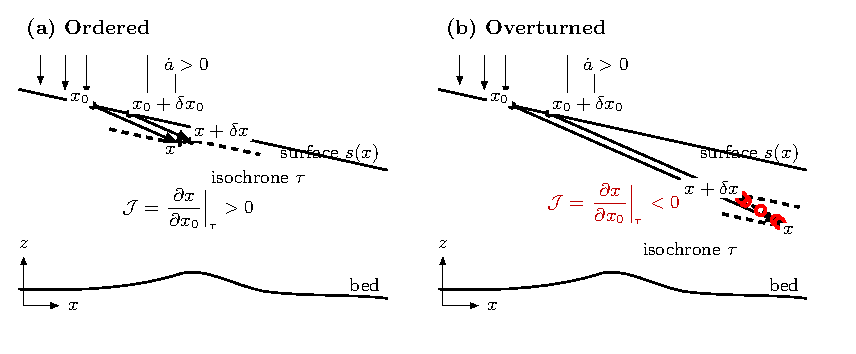
\includegraphics[width=\textwidth]{../figures/Figure1.pdf}
\caption{Material map for steady plane flow. Neighboring particles enter through the surface accumulation zone at \(x_0\) and \(x_0+\delta x_0\), follow distinct streamlines and reach positions separated by \(\delta x\) at the same age \(\tau\). The order Jacobian is the limit of \(\delta x/\delta x_0\). The curves enforce the kinematic requirements used in the derivation---surface origin, non-intersecting streamlines and transverse intersections with the isochrone---but are not a calculated Stokes solution.}
\label{fig:geometry}
\end{figure}

The streamfunction restricted to the surface is
\begin{equation}
\Psi(x)=\psi\bigl[x,s(x)\bigr].
\end{equation}
The steady surface kinematic condition is
\begin{equation}
 u_s s_x-\left.w\right|_{z=s(x)}=\dot a,
\label{eq:surfacekinematic}
\end{equation}
where \(u_s=u\bigl[x,s(x)\bigr]\). Differentiating \(\Psi\) with the chain rule, substituting Equation~\eqref{eq:streamfunction}, and then applying Equation~\eqref{eq:surfacekinematic} gives
\begin{equation}
\Psi'(x)
=\left.\psi_x\right|_{z=s(x)}+\left.\psi_z\right|_{z=s(x)}s_x
=-\left.w\right|_{z=s(x)}+u_ss_x
=\dot a(x)>0.
\label{eq:PsiPrime}
\end{equation}
The notation separates Eulerian position from material origin. The coordinate \(x\) is Eulerian: it identifies a fixed horizontal position in the steady velocity and age fields. The deposition coordinate \(x_0\) is a material-origin label that remains associated with a particle as it moves, although \(x_0\) alone labels a trajectory rather than a unique particle. At a specified age \(\tau\), \(x_0\) parameterizes the particles on an isochrone and therefore serves as the Lagrangian coordinate used below.

The streamfunction connects these descriptions. The increment \(\mathop{}\!\mathrm{d}\psi\) is the ice flux per unit width between neighboring streamlines. At the surface, this flux is \(\dot a_0\mathop{}\!\mathrm{d} x_0\), so larger accumulation places the same flux interval within a smaller deposition interval. Because \(\Psi'(x)>0\), every streamline label \(\psi\) has a unique deposition position \(x_0(\psi)\) satisfying
\begin{equation}
\Psi(x_0)=\psi,
\qquad
\frac{\mathop{}\!\mathrm{d} x_0}{\mathop{}\!\mathrm{d}\psi}=\frac{1}{\dot a_0},
\label{eq:x0psi}
\end{equation}
where \(\dot a_0\equiv\left.\dot a(x)\right|_{x=x_0}=\dot a(x_0)\) is the accumulation rate at deposition.

At fixed \(\psi\), Equation~\eqref{eq:age} gives
\begin{equation}
\left.\frac{\partial\tau}{\partial x}\right|_{\psi}=\frac{1}{u}.
\end{equation}
Consequently the age at \((x,\psi)\) is the travel time from deposition. Here, \(\xi\) is the horizontal coordinate of integration and \(z(\xi,\psi)\) is the elevation of the streamline labelled by \(\psi\):
\begin{equation}
\tau(x,\psi)=\int_{x_0(\psi)}^{x}
\frac{\mathop{}\!\mathrm{d}\xi}{u\left[\xi,z(\xi,\psi)\right]}.
\label{eq:traveltime}
\end{equation}
At fixed \(x\), Equation~\eqref{eq:streamfunction} implies
\begin{equation}
 z_{\psi}=\frac{1}{u}.
\label{eq:zpsi}
\end{equation}
Stratigraphic order compares travel times on neighboring streamlines, which are neighboring values of \(\psi\). We therefore differentiate Equation~\eqref{eq:traveltime} with respect to \(\psi\) at fixed downstream position. Using Equations~\eqref{eq:x0psi} and \eqref{eq:zpsi} gives
\begin{equation}
\tau_{\psi}
=-\frac{1}{\dot a_0u_{s0}}
-\int_{x_0}^{x}\frac{u_z}{u^3}\,\mathop{}\!\mathrm{d}\xi,
\label{eq:taupsi}
\end{equation}
where \(u_{s0}=u\left[x_0,s(x_0)\right]\) is the horizontal speed at deposition. The first term records the separation imposed at deposition; the integral records the subsequent differential travel time between neighboring streamlines.

\subsection{Exact order theorem}

We now use the material-origin coordinate to determine whether an isochrone retains its depositional ordering. Curvature alone is insufficient because a strongly curved isochrone can remain a single-valued depth surface and preserve the sequence of particles established at deposition. At fixed age, increasing \(x_0\) selects particles deposited successively farther downstream. Their order is preserved while their present horizontal position \(x\) also increases with \(x_0\); a vertical tangent occurs when this horizontal separation vanishes, and overturning begins when its sign reverses.

\medskip
\noindent\textbf{Definition 1 (Isochrone-order Jacobian).}
The isochrone-order Jacobian is
\begin{equation}
\mathcal{J}(x,x_0)
=\left.\frac{\partial x}{\partial x_0}\right|_{\tau}.
\label{eq:Jdefinition}
\end{equation}
It measures whether particles deposited in increasing order of \(x_0\) remain in increasing downstream order on an equal-age surface.

\medskip
\noindent\textbf{Theorem 1 (Cumulative order criterion).}
Under assumptions (A1)--(A4), the isochrone-order Jacobian is
\begin{equation}
\boxed{
\mathcal{J}
=\frac{u(x,z)}{u_{s0}}
\left(
1+\dot a_0u_{s0}
\int_{x_0}^{x}\frac{u_z}{u^3}\,\mathop{}\!\mathrm{d}\xi
\right).
}
\label{eq:Jexact}
\end{equation}
It is also related exactly to the vertical age gradient by
\begin{equation}
\boxed{\mathcal{J}=-\dot a_0\tau_z.}
\label{eq:Jage}
\end{equation}
Hence \(\mathcal{J}>0\) denotes ordered stratigraphy, \(\mathcal{J}=0\) a vertical tangent, and \(\mathcal{J}<0\) an overturned limb.

\medskip
\noindent\textit{Proof.}
At fixed age, differentiation of \(\tau(x,\psi)\) gives
\begin{equation}
\left.\frac{\partial x}{\partial\psi}\right|_{\tau}
=-\frac{\tau_{\psi}}{\tau_x|_{\psi}}
=-u\tau_{\psi}.
\end{equation}
Multiplication by \(\mathop{}\!\mathrm{d}\psi/\mathop{}\!\mathrm{d} x_0=\dot a_0\) and substitution of Equation~\eqref{eq:taupsi} gives Equation~\eqref{eq:Jexact}. At fixed \(x\), \(\tau_z=\tau_{\psi}\psi_z=u\tau_{\psi}\), which gives Equation~\eqref{eq:Jage}. \hfill\(\square\)

The correction of annual-layer thickness for cumulative ice deformation goes back at least to \citet{Nye1963} and \citet{DansgaardJohnsen1969}. In the present notation, the vertical thinning function \(\lambda_z\) is the current vertical thickness of an infinitesimal age layer divided by its ice-equivalent thickness at deposition. For an ordered layer, a positive age increment \(\mathop{}\!\mathrm{d}\tau\) corresponds to the present vertical thickness \(-\mathop{}\!\mathrm{d} z=-\mathop{}\!\mathrm{d}\tau/\tau_z\) and the initial thickness \(\dot a_0\mathop{}\!\mathrm{d}\tau\). Hence
\begin{equation}
\boxed{
\lambda_z
=-\frac{1}{\dot a_0\tau_z}
=\mathcal{J}^{-1},
\qquad \mathcal{J}>0.
}
\label{eq:thinningrelation}
\end{equation}
Thus \(\mathcal{J}\) is not a new independent state variable: in the ordered regime it is the inverse of the established vertical thinning function \citep{Parrenin2013,ParreninChungMartin2025}. Equation~\eqref{eq:Jage} provides its signed continuation through a vertical tangent. The standard positive thinning function diverges as \(\tau_z\rightarrow0\), whereas \(\mathcal{J}\) crosses zero regularly and records orientation reversal.

At deposition, \(x=x_0\), \(u=u_{s0}\), and \(\mathcal{J}=1\). At the first vertical tangent, \(\tau_z=0\), but the material curve remains regular. Inverting Equation~\eqref{eq:agepsiJacobian} shows that
\begin{equation}
\left.\frac{\partial z}{\partial x_0}\right|_{\tau}
=\dot a_0\tau_x.
\end{equation}
When \(\mathcal{J}=0\), Equation~\eqref{eq:age} gives \(\tau_x=1/u\), and therefore
\begin{equation}
\left.\frac{\partial z}{\partial x_0}\right|_{\tau,\mathcal{J}=0}
=\frac{\dot a_0}{u}>0.
\end{equation}
The divergence of the conventional slope \(m=\mathop{}\!\mathrm{d} z/\mathop{}\!\mathrm{d} x\) at overturning is therefore a coordinate singularity, not a singularity of the layer itself.

\subsection{Positive and reverse shear budgets}

Define
\begin{equation}
 u_z^+=\max(u_z,0),
 \qquad
 u_z^-=\max(-u_z,0),
\end{equation}
and the dimensionless cumulative contributions
\begin{align}
\mathcal{P}(x,x_0)
&=\dot a_0u_{s0}
\int_{x_0}^{x}\frac{u_z^+}{u^3}\,\mathop{}\!\mathrm{d}\xi,
\label{eq:Pdef}\\
\mathcal{R}(x,x_0)
&=\dot a_0u_{s0}
\int_{x_0}^{x}\frac{u_z^-}{u^3}\,\mathop{}\!\mathrm{d}\xi.
\label{eq:Rdef}
\end{align}
Equation~\eqref{eq:Jexact} becomes
\begin{equation}
\boxed{
\mathcal{J}=\frac{u}{u_{s0}}\mathcal{B},
\qquad
\mathcal{B}\equiv1+\mathcal{P}-\mathcal{R}.
}
\label{eq:JPR}
\end{equation}
The dimensionless factor \(\mathcal{B}\) is an order budget: deposition contributes the initial value one, normal shear adds \(\mathcal{P}\), and reverse shear subtracts \(\mathcal{R}\). Because \(u/u_{s0}>0\), the necessary-and-sufficient condition for preservation of horizontal order is
\begin{equation}
\boxed{\mathcal{R}<1+\mathcal{P}.}
\label{eq:ordercondition}
\end{equation}
The first vertical tangent occurs at
\begin{equation}
\boxed{\mathcal{R}=1+\mathcal{P},}
\label{eq:verticalcondition}
\end{equation}
and overturning occurs when \(\mathcal{R}>1+\mathcal{P}\).

The unit term in Equations~\eqref{eq:JPR}--\eqref{eq:verticalcondition} represents the initial ordering imposed at deposition. Positive \(u_z\), the usual surface-fast glacier profile, adds to the budget. Reverse shear must remove both contributions. Thus a local region with \(u_z<0\) is not itself a fold criterion.

In travel-time coordinates, \(\mathop{}\!\mathrm{d} x=u\,\mathop{}\!\mathrm{d} t\), so
\begin{equation}
\mathcal{R}
=\dot a_0u_{s0}
\int_0^T\frac{u_z^-}{u^2}\,\mathop{}\!\mathrm{d} t.
\label{eq:Rtime}
\end{equation}
where \(T\) is the travel time from deposition to the point of interest. Reverse shear is amplified by residence time and by slow horizontal motion. This weighting explains why local extrusion in fast throughflow may leave stratigraphic order unchanged, while modest reverse shear near stagnation can dominate the order budget.

\medskip
\noindent\textbf{Corollary 1 (Monotonic-shear result).}
If \(u_z\geq0\) everywhere along a trajectory, then \(\mathcal{R}=0\), \(\mathcal{J}>0\), and the steady isochrone cannot overturn.

This corollary is the physical-coordinate statement of the no-overturning result in Appendix A of \citet{ParreninHindmarsh2007}. It is sufficient, not necessary. Equation~\eqref{eq:ordercondition} permits finite intervals of reverse shear provided their cumulative weighted contribution remains below the order budget. Figure~\ref{fig:budget} summarizes the three contributions and the point at which the budget reaches zero.

\begin{figure}[t]
\centering
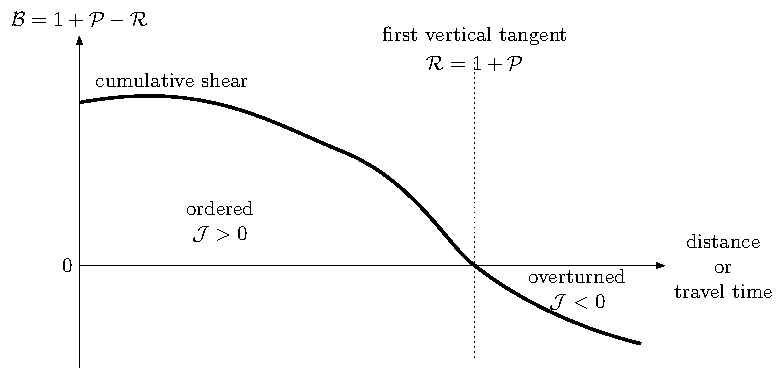
\includegraphics{../figures/Figure2.pdf}
\caption{Conceptual order budget. The sign of \(\mathcal{B}=1+\mathcal{P}-\mathcal{R}\) is the sign of the order Jacobian. Local reverse shear need not cause overturning; a vertical tangent appears only after cumulative reverse shear removes the initial depositional contribution and the accumulated normal-shear contribution.}
\label{fig:budget}
\end{figure}

\subsection{Relation to the Parrenin--Hindmarsh path factor}

\citet{ParreninHindmarsh2007} used a normalized streamfunction and logarithmic flux coordinates. For two neighboring particles, their Appendix A gives a mapping of the form
\begin{equation}
\delta\pi=(1-\alpha)\,\delta\pi_0,
\end{equation}
where \(\pi_0\) and \(\pi\) are their logarithmic flux coordinates at deposition and at the point of interest, respectively, and \(\alpha\) is their path-history factor. An isochrone exceeds vertical when \(\alpha>1\). Their present and surface-origin coordinates are monotone functions of \(x\) and \(x_0\) wherever assumptions (A2)--(A3) hold. Consequently,
\begin{equation}
\operatorname{sgn}(1-\alpha)
=\operatorname{sgn}\!\left(
\left.\frac{\partial x}{\partial x_0}\right|_{\tau}
\right)
=\operatorname{sgn}(\mathcal{J})
=\operatorname{sgn}(-\tau_z).
\label{eq:PHsign}
\end{equation}
The present result is therefore not an independent no-overturning theorem. Nor is \(\mathcal{J}\) independent of the established thinning variable: Equation~\eqref{eq:thinningrelation} identifies it as the signed inverse vertical-thinning factor. The contribution of the physical-space representation is that it exposes the positive and negative parts of vertical shear, remains regular at the first vertical tangent and can be evaluated directly from a numerical velocity field.

\section{Full-Stokes constraints on isochrone order}

\subsection{Exact stress decomposition of vertical shear}

The order theorem is kinematic. To determine whether glacier mechanics forces Equation~\eqref{eq:ordercondition} to hold, consider steady, isothermal or thermomechanically prescribed, isotropic generalized-Newtonian Stokes flow,
\begin{align}
\nabla\cdot\bm{u}&=0,
\label{eq:mass}\\
-\nabla p+\nabla\cdot\bm{\tau}+\rho\bm{g}&=\bm{0},
\label{eq:momentum}\\
\bm{\tau}&=2\eta\bm{D},
\qquad
\bm{D}=\tfrac12\left(\nabla\bm{u}+\nabla\bm{u}^{\mathsf T}\right),
\qquad \eta>0.
\label{eq:rheology}
\end{align}
Here, \(p\) is pressure, \(\rho\) is ice density, \(\bm{g}\) is gravitational acceleration, \(\bm{\tau}\) is deviatoric stress, \(\bm{D}\) is the strain-rate tensor and \(\eta>0\) is the scalar effective viscosity. The viscosity may depend on temperature and effective strain rate. Anisotropic rheology is discussed separately below.

With \(z\) vertical and gravity having no horizontal component, the horizontal momentum equation is
\begin{equation}
-p_x+\tau_{xx,x}+\tau_{xz,z}=0.
\label{eq:xmomentum}
\end{equation}
Write
\begin{equation}
p=p_{\mathrm{atm}}+\rho g(s-z)+p_{\mathrm{nh}},
\end{equation}
where \(g=|\bm{g}|\), \(p_{\mathrm{atm}}\) is atmospheric pressure and \(p_{\mathrm{nh}}\) contains all nonhydrostatic pressure, including the finite-slope surface correction. Integrating Equation~\eqref{eq:xmomentum} downward from the free surface, with \(\zeta\) as the vertical coordinate of integration, gives
\begin{equation}
\tau_{xz}(x,z)
=\tau_{xz}^{s}
-\rho g s_x(s-z)
+\int_z^s\left(\tau_{xx,x}-p_{\mathrm{nh},x}\right)\,\mathop{}\!\mathrm{d}\zeta.
\label{eq:tauxzint}
\end{equation}
Because \(\tau_{xz}=\eta(u_z+w_x)\),
\begin{equation}
\boxed{
 u_z
 =\underbrace{\frac{\rho g(s-z)(-s_x)}{\eta}}_{G}
 +\underbrace{
 \left[
 -w_x+\frac{\tau_{xz}^{s}}{\eta}
 +\frac{1}{\eta}\int_z^s
 \left(\tau_{xx,x}-p_{\mathrm{nh},x}\right)\,\mathop{}\!\mathrm{d}\zeta
 \right]}_{R_{\mathrm{FS}}}.
}
\label{eq:uzdecomp}
\end{equation}
where the superscript \(s\) denotes surface stress. For a surface descending downstream, \(s_x\leq0\), the gravity-driven term \(G\) is nonnegative and favors order preservation. The residual \(R_{\mathrm{FS}}\) contains the full-Stokes effects omitted from the shallow-ice shear balance: gradients of vertical velocity, longitudinal stress, nonhydrostatic pressure and the Cartesian surface shear-stress component.

Substitution into Equation~\eqref{eq:Jexact} gives
\begin{equation}
\mathcal{J}=\frac{u}{u_{s0}}
\left(1+\mathcal{G}+\mathcal{F}\right),
\label{eq:Jfullstokes}
\end{equation}
with
\begin{align}
\mathcal{G}&=\dot a_0u_{s0}
\int_{x_0}^{x}\frac{G}{u^3}\,\mathop{}\!\mathrm{d}\xi\geq0,
\label{eq:Ggrav}\\
\mathcal{F}&=\dot a_0u_{s0}
\int_{x_0}^{x}\frac{R_{\mathrm{FS}}}{u^3}\,\mathop{}\!\mathrm{d}\xi.
\label{eq:Gfs}
\end{align}
The exact full-Stokes condition for a vertical or overturned isochrone is
\begin{equation}
\boxed{
\mathcal{F}\leq-\left(1+\mathcal{G}\right).
}
\label{eq:FSfailure}
\end{equation}
A conservative sufficient condition for no overturning is
\begin{equation}
\boxed{
\dot a_0u_{s0}
\int_{x_0}^{x}
\frac{\left[R_{\mathrm{FS}}\right]_{-}}{u^3}\,\mathop{}\!\mathrm{d}\xi<1.
}
\label{eq:FSsufficient}
\end{equation}
This inequality discards all positive contributions, including gravity-driven shear, and is therefore stronger than necessary but easy to test.

\subsection{There is no universal full-Stokes sign theorem}

Neither incompressibility nor the Stokes equations fixes the sign of \(u_z\). The constitutive relation constrains \(u_z+w_x\), while longitudinal stress and nonhydrostatic pressure can alter the Cartesian vertical gradient of horizontal speed. Analytical rough-bed solutions predict local velocity maxima and minima, and therefore regions with \(u_z<0\), even for gravity-driven linear viscous flow \citep{Gudmundsson1997linear}. The historical extrusion-flow literature likewise shows that surface-fast velocity profiles are not a pointwise theorem of full-Stokes mechanics \citep{Waddington2010}.

At stronger roughness, the one-way-flow assumption itself can fail. \citet{Gudmundsson1997nonlinear} found separated secondary circulation in troughs of sufficiently steep sinusoidal beds. \citet{Moffatt1964} considered the local similarity solution near a sharp corner. For two stationary rigid planes, the similarity exponent becomes complex when the included angle is less than approximately \(146^{\circ}\); the resulting oscillation in \(\log r\) gives a nested sequence of closed, counter-rotating streamlines. \citet{MeyerCreyts2017} extended this corner-flow mechanism to Glen-law ice in subglacial mountain valleys and showed that oblique flow can produce three-dimensional eddies.

The conditions for Moffatt eddies and overturned steady isochrones are not the same. Moffatt eddies require a recirculating corner-flow mode. Isochrone overturning under assumptions (A1)--(A4) instead requires the open-trajectory order budget to reach zero. The circular-arc bed calculation in Figure~\ref{fig:positiveboundary} has \(u>0\) along every plotted trajectory and therefore overturns without an eddy. Conversely, a closed streamline cannot carry the steady, surface-sourced age field assumed here. Integrating Equation~\eqref{eq:age} around an orbit of period \(T>0\) would give
\begin{equation*}
\tau(T)-\tau(0)
=
\int_0^T\frac{\mathrm{D}\tau}{\mathrm{D}t}\,\mathop{}\!\mathrm{d} t
=T,
\end{equation*}
although the orbit returns to the same point and would require \(\tau(T)=\tau(0)\). A Moffatt eddy may deform inherited layers or contain ice supplied by another boundary, but it does not satisfy the unique surface-origin construction. Thus, a Moffatt eddy is neither necessary nor, within the present age problem, sufficient for an overturned surface-deposited isochrone.

The distinction between local extrusion and cumulative order reversal is central. Published rough-bed solutions establish that \(u_z\) can be negative. They do not, by that fact alone, establish that \(\mathcal{R}\) reaches \(1+\mathcal{P}\). The latter is an order-one integrated threshold.

\section{Regimes that preserve order}

\subsection{Shallow-ice flow}

Under the conventional shallow-ice approximation,
\begin{equation}
\tau_{xz}\simeq-\rho g(s-z)s_x.
\label{eq:SIAstress}
\end{equation}
For downstream flow with \(s_x<0\), \(\tau_{xz}>0\). An isotropic Glen-type rheology gives \(u_z\) with the same sign as \(\tau_{xz}\), while leading-order basal sliding contributes a depth-independent horizontal speed \citep{CuffeyPaterson2010}. Therefore
\begin{equation}
 u_z\geq0,
 \qquad \mathcal{R}=0,
 \qquad \mathcal{J}>0.
\label{eq:SIAorder}
\end{equation}
A fixed bed obstacle can produce arches, troughs and finite curvature in shallow-ice stratigraphy, but it cannot overturn a steady isochrone under these assumptions.

\subsection{Regular thin-film full-Stokes flow}

Let
\begin{equation}
\varepsilon=\frac{H}{L}\ll1
\end{equation}
be the aspect ratio of a smooth glacier. Higher-order glacier models reproduce the Stokes solution to second order in \(\varepsilon\) under their regular asymptotic assumptions, including a range of basal slip regimes \citep{Blatter1995,SchoofHindmarsh2010}. Suppose the non-shallow contribution scales as
\begin{equation}
R_{\mathrm{FS}}=O\left(\varepsilon^2\frac{U}{H}\right)
\label{eq:RFSscale}
\end{equation}
through a region of length \(L=H/\varepsilon\), and suppose \(u\) remains comparable to \(U\). Then
\begin{equation}
\mathcal{F}=O\left(\frac{\dot a}{U}\varepsilon\right).
\label{eq:GFSscale}
\end{equation}
Thus small regular full-Stokes corrections cannot erase the initial depositional contribution when
\begin{equation}
\frac{\dot a}{U}\varepsilon\ll1.
\label{eq:thinorder}
\end{equation}
This is an asymptotic sufficient regime, not a uniform theorem. The approximation can break down near divides, abrupt sliding transitions, contact zones, steep obstacles, very slow flow or other regions where the thin-film expansion is singular or nonuniform.

\subsection{A sufficient bound for a localized obstacle}

The cumulative criterion yields a direct obstacle bound without requiring pointwise monotonic shear.

\medskip
\noindent\textbf{Proposition 1 (Localized reverse-shear bound).}
Suppose reverse shear is confined to a trajectory segment of horizontal length \(\ell\). On that segment, assume
\begin{equation}
 u\geq U_{\min}>0,
 \qquad
 u_{s0}\leq U_{\mathrm{dep}},
 \qquad
 u_z^-\leq \dot\gamma_{\mathrm{rev}},
\label{eq:boundassumptions}
\end{equation}
where \(U_{\min}\) is the minimum horizontal speed on the segment, \(U_{\mathrm{dep}}\) bounds the horizontal speed at deposition, and \(\dot\gamma_{\mathrm{rev}}\) bounds the reverse vertical shear rate. Then
\begin{equation}
\boxed{
\mathcal{R}\leq
\frac{\dot a_0U_{\mathrm{dep}}\dot\gamma_{\mathrm{rev}}\ell}
{U_{\min}^{3}}.
}
\label{eq:obstaclebound}
\end{equation}
A sufficient condition for no overturning is that the right-hand side be less than one.

\medskip
\noindent\textit{Proof.}
Substitute Equation~\eqref{eq:boundassumptions} into Equation~\eqref{eq:Rdef} and bound the integral by its maximum integrand multiplied by \(\ell\). \hfill\(\square\)

For an isolated obstacle whose horizontal and vertical influence scales are both \(O(H)\), with non-stagnant throughflow,
\begin{equation}
\mathcal{R}=O\left(\frac{\dot a}{U}\right).
\label{eq:isolatedscale}
\end{equation}
In a typical interior or flank setting where \(U\gg\dot a\), an isolated fixed bump can create local extrusion and visible draping while remaining far from the reverse-shear value required for a vertical tangent. More generally, setting the right-hand side of Equation~\eqref{eq:obstaclebound} equal to one and solving for length gives
\begin{equation}
\ell
\gtrsim
\frac{U_{\min}^{3}}
{\dot a_0U_{\mathrm{dep}}\dot\gamma_{\mathrm{rev}}}.
\label{eq:lengththreshold}
\end{equation}
Slow throughflow reduces this required length through the \(U_{\min}^{3}\) numerator. For scale, take \(\dot a_0=0.05~\mathrm{m\,yr^{-1}}\), \(U_{\mathrm{dep}}=10~\mathrm{m\,yr^{-1}}\), \(\dot\gamma_{\mathrm{rev}}=0.01~\mathrm{yr^{-1}}\) and \(\ell=1~\mathrm{km}\). Equation~\eqref{eq:obstaclebound} gives \(\mathcal{R}\leq0.005\) when \(U_{\min}=10~\mathrm{m\,yr^{-1}}\), which rules out overturning under these assumed bounds. With \(U_{\min}=1~\mathrm{m\,yr^{-1}}\), the bound is \(\mathcal{R}\leq5\) and no longer rules it out.

Equation~\eqref{eq:obstaclebound} makes precise why ``flow over a bump cannot fold an isochrone'' is often a good glacier approximation but not a universal Stokes theorem. The approximation depends on non-stagnant flow, a localized deformation zone and a small accumulation-to-speed ratio.

\subsection{First-order cancellation over periodic roughness about plug flow}

A second reason that fixed roughness may have weak cumulative effect is cancellation, but the result requires a plug-flow background. Let
\begin{equation}
 u(x,z;\epsilon_b)=U_b+\epsilon_b u_1(x,z)+O(\epsilon_b^2),
 \qquad U_b>0,
\label{eq:plugperturbation}
\end{equation}
where \(\epsilon_b\) is a small amplitude parameter, \(U_b>0\) is spatially uniform, \(u_1\) is periodic in \(x\), and \(k\) is its wavenumber. The perturbation has wavelength \(2\pi/k\) and zero horizontal mean at each elevation. Along the unperturbed trajectory \(z=z_0\),
\begin{equation}
\frac{u_z}{u^3}
=\epsilon_b\frac{u_{1,z}(x,z_0)}{U_b^3}+O(\epsilon_b^2).
\label{eq:periodicshear}
\end{equation}
Therefore, over one complete wavelength,
\begin{equation}
\int_{x}^{x+2\pi/k}\frac{u_z}{u^3}\,\mathop{}\!\mathrm{d}\xi=O(\epsilon_b^2).
\label{eq:periodiccancel}
\end{equation}
The appendix on first-order periodic cancellation gives the expansion leading to Equation~\eqref{eq:periodiccancel}. The perturbative frictionless rough-bed solution of \citet{Gudmundsson1997linear} has this plug-flow structure: local extrusion occurs, but its first-order stoss- and lee-side contributions cancel over a complete symmetric wavelength.

Cancellation is not guaranteed for a sheared background, a solitary asymmetric obstacle, a finite path ending mid-cycle, strongly nonlinear roughness or near-stagnant trajectories. Equation~\eqref{eq:periodiccancel} is therefore a restricted asymptotic result, not a general symmetry theorem.

\section{Trajectory diagnostic for full-Stokes models}

The order criterion can be evaluated without explicitly solving the age equation or advecting a dense family of isochrones. Start trajectories in a surface accumulation zone and record \(x_0\), \(\dot a_0\) and \(u_{s0}\). With \(t\) denoting time since deposition, integrate along each trajectory
\begin{align}
\frac{\mathop{}\!\mathrm{d} x}{\mathop{}\!\mathrm{d} t}&=u,
&
\frac{\mathop{}\!\mathrm{d} z}{\mathop{}\!\mathrm{d} t}&=w,
\label{eq:trajectory}\\
\frac{\mathop{}\!\mathrm{d}\mathcal{P}}{\mathop{}\!\mathrm{d} t}
&=\dot a_0u_{s0}\frac{u_z^+}{u^2},
&
\frac{\mathop{}\!\mathrm{d}\mathcal{R}}{\mathop{}\!\mathrm{d} t}
&=\dot a_0u_{s0}\frac{u_z^-}{u^2},
\label{eq:PRode}
\end{align}
with \(\mathcal{P}(0)=\mathcal{R}(0)=0\). Then
\begin{equation}
\boxed{
\mathcal{J}(t)=\frac{u(t)}{u_{s0}}
\left[1+\mathcal{P}(t)-\mathcal{R}(t)\right].
}
\label{eq:Jdiagnostic}
\end{equation}
The diagnostic is
\begin{equation}
\min_t\left[1+\mathcal{P}(t)-\mathcal{R}(t)\right]
\begin{cases}
>0, & \text{order preserved},\\
=0, & \text{first vertical tangent},\\
<0, & \text{overturned steady isochrone}.
\end{cases}
\label{eq:numericaltest}
\end{equation}

A robust implementation should include four checks. First, compare Equation~\eqref{eq:Jdiagnostic} with \(-\dot a_0\tau_z\) from an independently solved steady age equation. Second, advect at least one pair of neighboring particles to verify the sign of \(\partial x/\partial x_0|_{\tau}\). Third, stop the downstream-coordinate integration when \(u\) approaches zero and diagnose recirculation with the full trajectory topology. Fourth, compute \(u_z\) using the finite-element gradient rather than differencing noisy interpolated velocities. Separate storage of \(\mathcal{P}\) and \(\mathcal{R}\) is preferable to integrating their difference because large compensating contributions can otherwise obscure numerical error.

For transient flow, Equation~\eqref{eq:Jdiagnostic} is not valid because the steady travel-time representation fails. The corresponding calculation should integrate the deformation of the two-parameter deposition map through time. Nevertheless, the steady order budget remains useful as a baseline and as a diagnostic applied to quasi-steady snapshots.

\section{Full-Stokes numerical example}

We test whether a steady full-Stokes velocity field can generate a recumbent fold from ordered surface deposition without an imposed internal disturbance. The calculation uses a linear sliding law and gravity as its mechanical driving force. It is an idealized existence example, not a reconstruction of Allan Hills or another old-ice site.

The two-dimensional domain has a flat upper surface and a bed whose vertical cross section is a circular arc of radius \(250~\mathrm{m}\). Its maximum thickness is \(150~\mathrm{m}\), and it is truncated by vertical cuts where the ice has positive thickness. Ice is incompressible and linear viscous, with \(\eta=2.5\times10^8~\mathrm{Pa\,yr}\) and \(\rho=917~\mathrm{kg\,m^{-3}}\). Gravity acts at a mean surface slope of \(0.05~\mathrm{rad}\). We implemented the weak form in Firedrake version \texttt{0.13.0+11207.g7ed6ff028}, generated curved unstructured meshes with Gmsh, imposed basal impermeability with symmetric Nitsche terms and solved the mixed system with the MUMPS direct solver. Velocity and pressure use Taylor--Hood elements, with quadratic velocity and linear pressure.

During model development, OpenAI \texttt{5.6-sol} was used to search candidate boundary conditions, including bed geometry, for a clear example of steady overturning. The final geometry and boundary conditions were then evaluated using the governing equations, mechanical power balance, trajectory topology and mesh-refinement tests reported here.

The bed is impermeable and obeys the linear sliding law
\begin{equation}
u_t=C\tau_b,
\qquad
u_n=0,
\qquad
\tau_b=-\bm{t}\mathbin{\cdot}\bm{\sigma}\bm{n},
\label{eq:linearsliding}
\end{equation}
where \(u_t\) and \(u_n\) are the tangential and normal basal velocities, \(\tau_b\) is the resisting basal shear stress, and \(C=10^{-5}~\mathrm{m\,yr^{-1}\,Pa^{-1}}\) is the mobility. Because \(C>0\), Equation~\eqref{eq:linearsliding} dissipates mechanical energy. The surface is traction free. Each lateral boundary has the hydrostatic traction \(-\rho g\cos\theta(-z)\bm{n}\), where \(\theta\) is the mean surface slope. The accumulation rate required to keep the surface fixed is diagnosed as \(\dot a=-\left.w\right|_{z=0}\), and particles are introduced only where \(\dot a>0\).

The numerical isochrones are generated from the deposition boundary. At age zero, a particle labelled by \(x_0\) is placed at \([x_0,0]^{\mathsf T}\). Integrating the steady velocity for a common age \(\tau\) gives the material curve \([x(x_0,\tau),z(x_0,\tau)]^{\mathsf T}\). We do not initialize an internal layer, wrinkle or fold. A negative value of \(\left.\partial x/\partial x_0\right|_\tau\) therefore measures order reversal generated between deposition and the plotted isochrone.

For the representative calculation, the ice is \(70~\mathrm{m}\) thick at both lateral boundaries. The boundaries together remove \(4.3\times10^2~\mathrm{Pa\,m^2\,yr^{-1}}\) of mechanical power per unit width, whereas gravity supplies \(4.63\times10^6~\mathrm{Pa\,m^2\,yr^{-1}}\). The lateral tractions therefore do not drive the flow. The deposition map first reaches \(\mathcal{J}=-0.20\) at \(1.374~\mathrm{kyr}\) (Figure~\ref{fig:positiveboundary}a--b). At that age, all 47 surface origins spanning \(25.9~\mathrm{m}\) remain within the domain, and horizontal speed has remained above \(0.143~\mathrm{m\,yr^{-1}}\). The same threshold is reached with \(23\)--\(92~\mathrm{m}\) of ice at both boundaries (Figure~\ref{fig:positiveboundary}c).

The flow is rotational but does not contain a Moffatt eddy. Horizontal speed remains positive along every plotted trajectory, so the streamlines are open. The fold forms because reverse shear rotates the surface-deposition map through vertical, not because particles circulate on a closed streamline. Neither a zero-thickness margin nor recirculation is required.

For the \(70~\mathrm{m}\) boundary-thickness case, meshes with nominal spacings of \(15\), \(10\), \(7.5\) and \(5~\mathrm{m}\) give \(\mathcal{J}=-0.20061\), \(-0.20053\), \(-0.20040\) and \(-0.20037\), respectively, at the first resolved threshold. The overturned interval and its age are therefore insensitive to mesh refinement at the reported precision.

\begin{figure}[t]
\centering
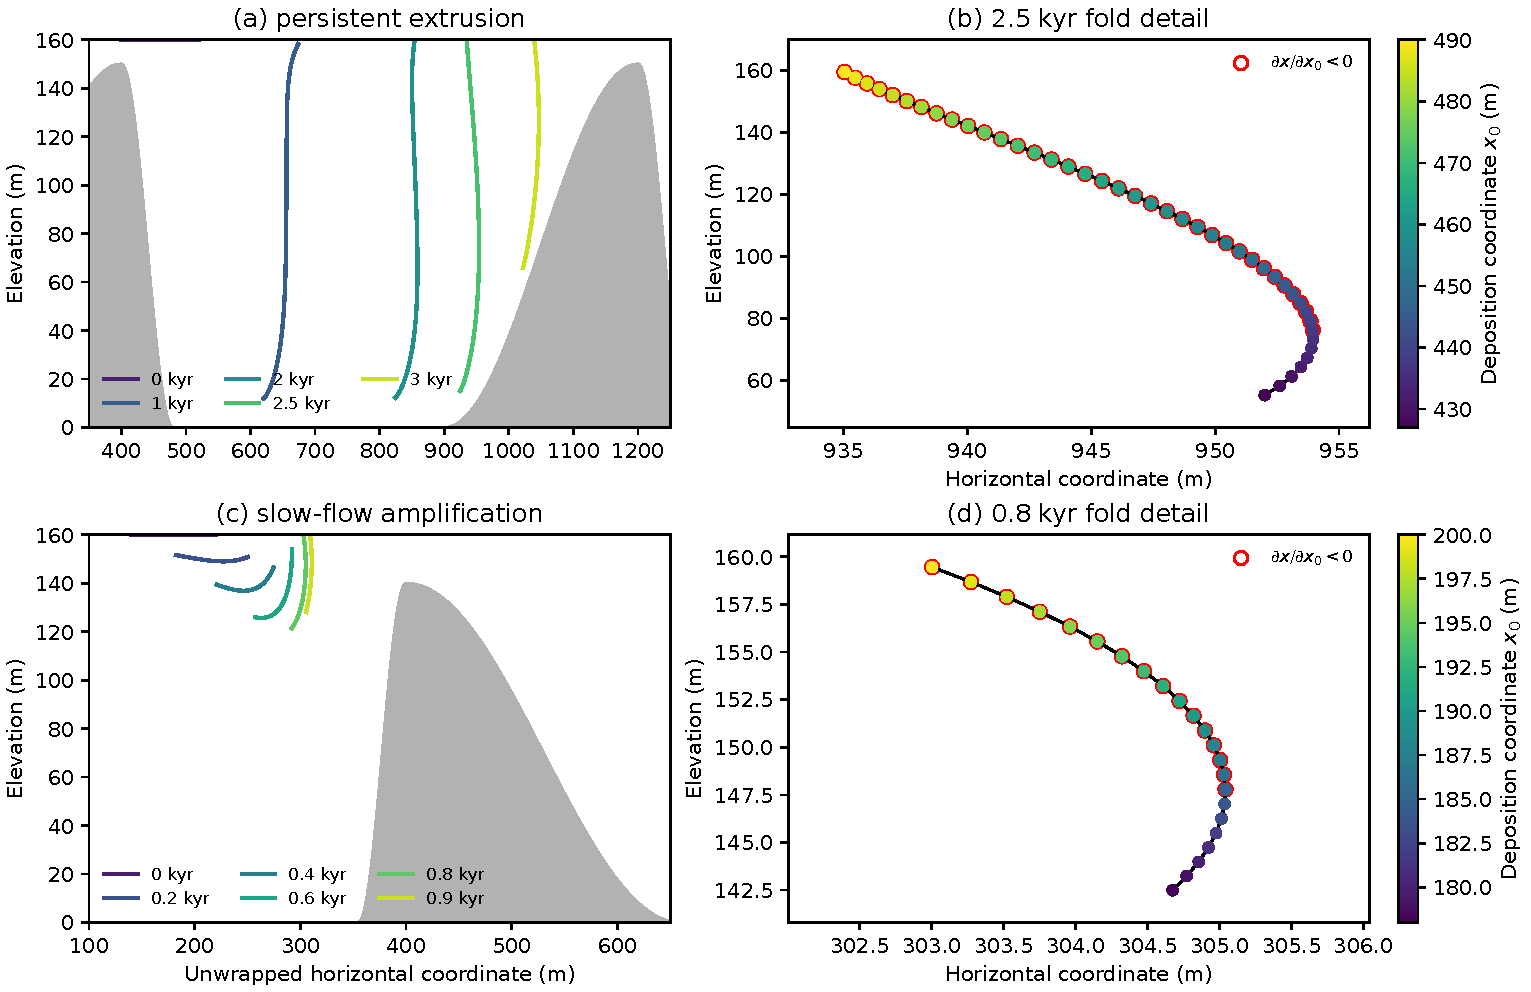
\includegraphics[width=\textwidth]{../figures/Figure3.pdf}
\caption{Gravity-driven order reversal with positive thickness at both lateral boundaries. The bed cross section is a circular arc with \(150~\mathrm{m}\) maximum ice thickness, and the bed obeys a linear sliding law; hydrostatic traction is applied on the open lateral cuts. (a) Isochrone evolution at \(0\), \(0.30\), \(0.60\), \(0.90\), \(1.15\) and \(1.374~\mathrm{kyr}\), for \(70~\mathrm{m}\) boundary thickness. Each curve consists of the same surface-deposition origins evaluated at a common age. (b) Detail at the final age, when the minimum order Jacobian is less than \(-0.20\). Color gives deposition coordinate \(x_0\), and open red circles mark \(\mathcal{J}<0\). (c) Age at which the same threshold is crossed as boundary thickness increases from \(23\) to \(92~\mathrm{m}\). All deposition origins remain in the domain at the plotted threshold.}
\label{fig:positiveboundary}
\end{figure}

The topographic relief is large and the rheology is linear viscous. The calculation establishes that a gravity-driven flow with a linear sliding law and positive lateral thickness can overturn a surface-generated isochrone; it does not establish that this mechanism produced the observed Allan Hills stratigraphy. Testing that hypothesis requires measured three-dimensional geometry, a basal traction model and source-to-core trajectories consistent with the observed surface mass balance.

\section{Discussion}

\subsection{Limits of the steady coordinate construction}

Within assumptions (A1)--(A4), cumulative reverse shear can overturn an isochrone when Equation~\eqref{eq:verticalcondition} is met. No boundary change is required. The extrusion-flow literature establishes local reverse shear, but does not evaluate this cumulative threshold. Variable density requires the mass-flux extension given in the appendix.

Stagnation and recirculation instead violate the coordinate construction. If \(u\) vanishes or reverses, downstream position no longer parameterizes a trajectory and the \(1/u\) and \(1/u^3\) integrals become singular. Time integration remains possible, but a closed streamline cannot have the unique surface origin assumed here. The Allan Hills model of \citet{Manos2026} approaches this limit: its near-stagnant basal flow remains nonzero, yet makes the order integral sensitive to small velocities.

Material sources also restrict the theorem. A trajectory may enter through accumulation and leave through surface ablation, but its deposition coordinate must be defined on the originating accumulation zone. Multiple surface sources or basal freeze-on require a more general label. Basal melting and ablation truncate layers, while freeze-on can add debris-bearing structures that are not surface-deposited isochrones \citep{LeysingerVieli2018,Holschuh2026}.

Changes in geometry or basal traction leave an inherited age field that differs from the steady age solution. Divide migration, traveling traction anomalies and former ice-stream configurations can therefore seed folds later amplified by shear \citep{JacobelBindschadler1993,JacobsonWaddington2005,Wolovick2014,WolovickCreyts2016,Franke2022,Jansen2024}. These mechanisms remain distinct from overturning generated continuously in a fixed velocity field.

Finally, Equation~\eqref{eq:uzdecomp} assumes isotropic scalar viscosity and the order theorem is two-dimensional. Fabric and rheological heterogeneity can actively generate folds \citep{Alley1997,ThorsteinssonWaddington2002,Bons2016,Bons2025}, and convergent anisotropic flow occurs in both radar observations and models \citep{Ross2020,MartinGudmundssonPritchardGagliardini2009}. In three dimensions, the relevant quantity is the two-dimensional Jacobian mapping a surface deposition patch to an equal-age surface. The scalar \(\mathcal{J}\) applies only within a coherent flow tube with negligible cross-flow.

\subsection{Implications for old-ice sites}

Allan Hills approaches several limits of the two-dimensional calculation. Ice rises into an ablation zone above steep nunatak topography \citep{Spaulding2012,Kehrl2018,Stoll2026}. \citet{Manos2026} predict nearly stagnant basal ice upstream of the nunatak: the bottom \(20~\mathrm{m}\) averages \(0.4\)--\(0.5~\mathrm{mm\,yr^{-1}}\), with local speeds of order micrometres per year, compared with \(46\)--\(49~\mathrm{mm\,yr^{-1}}\) in the Cul-de-sac. Such small \(u\) makes the \(u^{-3}\) order integral numerically sensitive. The modeled flow is also three-dimensional, with bridging stresses represented in two dimensions by the \(-w_x\) term in Equation~\eqref{eq:uzdecomp}. Finally, Cul-de-sac transport and geochemistry indicate a distinct accumulation environment. A three-dimensional, multi-source material map is therefore required there.

Observations constrain but do not determine this history. The \(69^{\circ}\) mean dip in ALHIC2302 remains below vertical \citep{Kirkpatrick2025}, and centimetre-scale folds in ALHIC1901 need not explain core-scale reversals \citep{Stoll2026}. The ALHIC1901 age--depth inversion implies \(\mathcal{J}<0\) through Equation~\eqref{eq:Jage} only if samples belong to one continuous surface-deposited layer family \citep{Shackleton2025}.

At Beyond EPICA, radar and flow modelling indicate strong basal thinning and possibly stagnant or disturbed ice \citep{Lilien2021,Chung2025BeyondEPICA}. Evaluating \(\mathcal{J}\) along trajectories would test whether steady flow preserves order above this basal unit.

The equations suggest four tests of an observed fold or age reversal.

\begin{enumerate}[leftmargin=*,label=(\arabic*)]
  \item \textbf{Steady geometry.} Evaluate \(\mathcal{P}\), \(\mathcal{R}\) and \(\mathcal{J}\) along source-to-core trajectories. A positive budget excludes steady overturning.
  \item \textbf{Flow topology and sources.} Test for stagnation, recirculation, freeze-on and multiple surface origins; these require the full material map.
  \item \textbf{Unsteady inheritance.} If steady flow preserves order, evaluate past changes in geometry, ablation and basal traction.
  \item \textbf{Active deformation.} If passive models underpredict folding, couple fabric and rheological heterogeneity to flow.
\end{enumerate}

In regular, shallow, non-stagnant flow, Equation~\eqref{eq:obstaclebound} favors a time-dependent or rheological mechanism. More general full-Stokes flow can overturn steady isochrones if reverse shear crosses the order threshold.


\subsection{Novelty and relationship to established theory}

The analysis builds on established components: the WBA local wrinkle criterion, finite-strain amplification \citep{JacobsonWaddington2004}, the Parrenin--Hindmarsh path factor and monotonic-shear result \citep{ParreninHindmarsh2007}, vertical thinning \citep{Parrenin2013,ParreninChungMartin2025} and rough-bed extrusion \citep{Gudmundsson1997linear}. Its theoretical contribution is to express signed inverse thinning as a positive--negative \(u_z/u^3\) budget. This physical-space form yields the full-Stokes residual threshold, localized-obstacle bound, periodic cancellation result and trajectory diagnostic.

The constructive contribution is a full-Stokes realization of order reversal from surface deposition. We are not aware of a previous calculation in which a time-independent glacier velocity carries an ordered deposition map to \(\mathcal{J}<0\) without an internal wrinkle. Here gravity drives the flow, a linear sliding law dissipates energy, lateral tractions are hydrostatic, and both lateral ice thickness and trajectory speed remain positive. The idealized circular-arc bed establishes a mechanical possibility, not a general topographic mechanism.

Applying the diagnostic to reconstructed Allan Hills flow would distinguish a positive budget, which excludes steady overturning, from a trajectory crossing \(\mathcal{J}=0\). Layer attitudes, age reversals and fabric provide independent tests.

\subsection{Limitations}

The analysis assumes a smooth two-dimensional velocity, isotropic scalar viscosity and one surface origin per trajectory. The obstacle bound requires externally supplied velocity and shear bounds, while periodic cancellation is only first order. Most importantly, \(\mathcal{J}\) diagnoses a continuous material isochrone. Faults, unconformities, freeze-on, multiple sources and unresolved three-dimensional geometry can also produce apparent age reversals. Steep specular limbs or debris-rich diffuse reflectors add ambiguity in radar data \citep{Holschuh2014,Holschuh2026}.

\section{Conclusions}

A steady two-dimensional isochrone preserves depositional order if and only if its signed order Jacobian remains positive (cf. Equation~\eqref{eq:Jexact}). The equivalent observable condition is \(\tau_z<0\) (Equation~\eqref{eq:Jage}), and in the ordered regime \(\mathcal{J}\) is the reciprocal of the established vertical thinning function (Equation~\eqref{eq:thinningrelation}). Pointwise surface-fast shear, \(u_z\geq0\), is sufficient but not necessary. The exact condition is the cumulative order budget \(\mathcal{R}<1+\mathcal{P}\) (Equation~\eqref{eq:ordercondition}).

Full-Stokes mechanics does not guarantee this condition for arbitrary glacier geometry. Gravity-driven shear favors order, but longitudinal stress, nonhydrostatic pressure and horizontal gradients of vertical velocity can generate reverse shear (cf. Equation~\eqref{eq:uzdecomp}). The shallow-ice regime preserves order (Equation~\eqref{eq:SIAorder}); non-stagnant localized obstacles and small-amplitude periodic roughness obey the more restricted results in Equations~\eqref{eq:obstaclebound} and \eqref{eq:periodiccancel}. Stagnation and recirculation invalidate the one-way coordinate construction.

The numerical example generates a recumbent isochrone directly from ordered surface deposition (Figure~\ref{fig:positiveboundary}). Gravity drives the flow, the bed obeys a linear sliding law, and the ice has positive thickness at both lateral boundaries. The horizontal velocity remains positive along the relevant trajectories, so the rotational flow is not a Moffatt eddy. This calculation establishes that steady full-Stokes flow can cross the order threshold under glaciological boundary conditions, although it does not show that such overturning is common.

For NSF COLDEX at Allan Hills, the next calculation is to integrate \(\mathcal{P}\), \(\mathcal{R}\) and \(\mathcal{J}\) along reconstructed source-to-core trajectories using Equations~\eqref{eq:trajectory}--\eqref{eq:Jdiagnostic}. A three-dimensional material map is required where cross-flow or multiple source regions are important. The same diagnostic can test stratigraphic order at continuous old-ice sites such as Beyond EPICA.

\section*{Data availability statement}
No new observational data are presented. The analytical results are fully specified by the equations in this manuscript. Executed notebooks contain the full-Stokes solves, trajectory calculations, numerical checks and figure generation and are available at \texttt{github.com/bradlipovsky/allan-hills-stratigraphy}.

\section*{Author contributions}
Bradley Paul Lipovsky developed the analysis and wrote the manuscript draft.

\section*{Competing interests}
To be completed by the author before submission.

\section*{Acknowledgements}
To be completed before submission. Support and contributions from NSF COLDEX and collaborating investigators should be documented here.

OpenAI Codex using GPT-5 and \texttt{5.6-sol} (available at \texttt{openai.com/codex}) was used from 3 to 29 August 2026 to assist with literature searches, drafting and revising manuscript text, LaTeX formatting, numerical-code development and the search for illustrative model geometries and boundary conditions. The author reviewed and revised all AI-assisted material, verified the cited sources, equations, code and numerical results, and takes full responsibility for the manuscript.

\bibliographystyle{igs}
\bibliography{references}

\appendix

\section{Inverse-coordinate identities}

Equation~\eqref{eq:agepsiJacobian} can be written
\begin{equation}
\begin{bmatrix}
\tau_x & \tau_z\\
\psi_x & \psi_z
\end{bmatrix}
\begin{bmatrix}
\mathop{}\!\mathrm{d} x\\
\mathop{}\!\mathrm{d} z
\end{bmatrix}
=
\begin{bmatrix}
\mathop{}\!\mathrm{d}\tau\\
\mathop{}\!\mathrm{d}\psi
\end{bmatrix},
\qquad
\det=1.
\end{equation}
The inverse transformation is
\begin{equation}
\begin{bmatrix}
\mathop{}\!\mathrm{d} x\\
\mathop{}\!\mathrm{d} z
\end{bmatrix}
=
\begin{bmatrix}
\psi_z & -\tau_z\\
-\psi_x & \tau_x
\end{bmatrix}
\begin{bmatrix}
\mathop{}\!\mathrm{d}\tau\\
\mathop{}\!\mathrm{d}\psi
\end{bmatrix}
=
\begin{bmatrix}
 u & -\tau_z\\
 w & \tau_x
\end{bmatrix}
\begin{bmatrix}
\mathop{}\!\mathrm{d}\tau\\
\mathop{}\!\mathrm{d}\psi
\end{bmatrix}.
\label{eq:inversemap}
\end{equation}
Therefore
\begin{equation}
 x_{\tau}|_{\psi}=u,
 \quad
 z_{\tau}|_{\psi}=w,
 \quad
 x_{\psi}|_{\tau}=-\tau_z,
 \quad
 z_{\psi}|_{\tau}=\tau_x.
\end{equation}
The first two identities state that advancing one unit in age at fixed streamline follows the velocity for one unit of time. The latter two specify the equal-age tangent. Multiplication by \(\mathop{}\!\mathrm{d}\psi/\mathop{}\!\mathrm{d} x_0=\dot a_0\) yields Equation~\eqref{eq:Jage} and the corresponding vertical tangent component.

\section{Extension to steady variable-density flow}

Below the firn, glacier ice is accurately treated as incompressible with nearly constant density. The coordinate construction extends to a steady variable-density flow satisfying
\begin{equation}
\nabla\cdot(\rho\bm{u})=0.
\end{equation}
Define the mass-flux streamfunction by
\begin{equation}
\rho u=\psi_z,
\qquad
\rho w=-\psi_x.
\end{equation}
Then
\begin{equation}
\begin{vmatrix}
\tau_x & \tau_z \\
\psi_x & \psi_z
\end{vmatrix}
=\rho(u\tau_x+w\tau_z)=\rho.
\end{equation}
The mapping remains nonsingular for \(\rho>0\), and the same order interpretation follows after replacing volume flux by mass flux. The constant-density formula used in the main text is therefore not conceptually tied to strict incompressibility, although the weights in the cumulative integral acquire density factors.

\section{First-order periodic cancellation about plug flow}

Let
\begin{equation}
 u(x,z;\epsilon_b)=U_b+\epsilon_b u_1(x,z)+O(\epsilon_b^2),
 \qquad U_b>0,
\end{equation}
where \(U_b\) is spatially uniform and \(u_1\) is periodic in \(x\) with wavelength \(2\pi/k\) and zero horizontal mean at each elevation. Then
\begin{equation}
 u_z=\epsilon_b u_{1,z}+O(\epsilon_b^2),
 \qquad
 u^{-3}=U_b^{-3}+O(\epsilon_b).
\end{equation}
Because the background integrand is identically zero, the \(O(\epsilon_b)\) displacement of the trajectory affects the integral only at \(O(\epsilon_b^2)\). Evaluating the first-order term along the unperturbed streamline \(z=z_0\) gives
\begin{equation}
\int_x^{x+2\pi/k}\frac{u_z}{u^3}\,\mathop{}\!\mathrm{d}\xi
=\frac{\epsilon_b}{U_b^3}
\int_x^{x+2\pi/k}u_{1,z}(\xi,z_0)\,\mathop{}\!\mathrm{d}\xi
+O(\epsilon_b^2)
=O(\epsilon_b^2),
\end{equation}
because differentiation with respect to \(z\) preserves the zero horizontal mean of \(u_1\). This establishes Equation~\eqref{eq:periodiccancel}. For a vertically sheared background, trajectory displacement can act on the nonzero background integrand at first order, so the cancellation does not follow without additional assumptions.

\end{document}
